% 中文 V2 独立入口；正文按 2026-10-21 Word 原文同步，使用 XeLaTeX 编译。
\documentclass[a4paper,11pt]{article}
\usepackage[UTF8,fontset=fandol,heading=true]{ctex}
\usepackage[margin=23mm]{geometry}
\usepackage{setspace}
\setstretch{1.25}
\usepackage{amsmath,amssymb}
\usepackage{graphicx}
\usepackage{booktabs,tabularx,array}
\usepackage{caption}
\usepackage{float}
\usepackage{placeins}
\usepackage{xcolor}
\usepackage[hidelinks]{hyperref}
\usepackage{authblk}
\setlength{\parindent}{2em}
\setlength{\parskip}{0.25em}
\setlength{\emergencystretch}{2em}
\captionsetup{font=small,labelfont=bf}
% 图占据单独浮动页时从正文顶端排起，避免上方大块留白。
\makeatletter
\setlength{\@fptop}{0pt}
\makeatother
\ctexset{section={format=\Large\bfseries},subsection={format=\large\bfseries}}
\newcommand{\authorinput}[1]{\textcolor{red!65!black}{\textbf{［待核实：#1］}}}
\newcommand{\IC}{\ensuremath{\mathrm{IC}_{50}}}

% 沿用原稿的作者姓名、顺序和单位，不推定本轮小组分工对应的作者贡献。
\author[1]{Xinge Xia}
\author[1]{Fan Wu}
\author[2]{Xianyou Duan}
\author[1]{Hongyi Chen}
\author[1]{Bingwen Feng*}
\affil[1]{College of Cyber Security, Jinan University, Guangzhou, China}
\affil[2]{College of Chemistry and Materials Science, Jinan University, Guangzhou, China}
\renewcommand{\Authfont}{\normalsize}
\renewcommand{\Affilfont}{\small}
\title{纳米硒细胞毒性预测的严格分组评估\\[0.3em]与 HUVEC 剂量—时间实验}
\date{中文 V2 修订稿\quad 2026 年 10 月 12 日\\\small * 通讯作者：bingwfeng@gmail.com}

\begin{document}
\maketitle
\begin{abstract}
纳米硒（SeNPs）细胞毒性预测需要区分同一研究内的拟合表现、跨文献泛化与新材料实验观测，材料化学信息能否在基础描述符之外提供稳定收益也需要独立检验。本研究采用通用纳米材料基准、历史纳米硒分组建模与新增人脐静脉内皮细胞（HUVEC）实验相结合的设计，在 434 条历史记录、24 个文献组上进行 5 折外层、3 折内层嵌套交叉验证，并比较化学增强、剂量—时间交互和固定预算迁移策略。无实测半数抑制浓度（\IC）输入的随机森林基础模型取得折外平均绝对误差 19.11 个百分点、均方根误差 24.12 个百分点和 $R^2=0.109$，新增化学描述符、显式交互项与迁移策略均未显示稳定的误差降低。

独立实验数据包含 9 种 SeNPs 在 HUVEC 中的 351 条报告值，覆盖 24、48、72 h 和 13 个浓度水平。在最高报告浓度 512 下，9 种材料的平均存活率由 24 h 的 59.81\% 降至 72 h 的 26.38\%，材料间差异也随评价条件而变化。27 条材料—时间曲线中，19 条可通过相邻点的对数浓度插值得到表观 \IC，8 条在测试范围内未达到 50\% 存活率。实验提供了剂量—时间响应与材料差异的描述性证据，但现有归档没有事先封存的逐条件模型预测，也未提供原始重复孔数据；浓度单位的含义和计量基准仍待核实。这些结果支持以严格评价和可追溯实验观测约束纳米硒毒性预测的应用范围，尚不足以证明新材料的前瞻预测精度或单一材料性质的因果作用。

\end{abstract}
\noindent\textbf{关键词：}纳米硒；细胞毒性；文献分组验证；前瞻盲法预测；HUVEC；剂量—时间响应

\section{引言}

纳米硒（selenium nanoparticles，SeNPs）的细胞毒性评价需要同时考虑材料性质与暴露条件，单个粒径或单一浓度下的实验结果难以覆盖不同使用情境。已有细胞与动物研究显示，SeNPs 的生物学效应并不能仅由“纳米硒”这一材料名称概括，材料修饰与暴露水平都需要纳入安全性评价\cite{wang2020prooxidation,lunkov2023chitosan}。对不同表面修饰材料获取剂量—时间响应，有助于明确观测差异出现在哪些条件下，也为预测模型提供直接的评价对象。

文献数据为计算毒理学提供了覆盖多种材料和细胞体系的研究基础。Gul 等整合纳米颗粒材料、细胞和实验属性，通过关联规则分析研究细胞毒性之间的关系 \cite{gul2021association}；Masarkar 等进一步利用随机森林开展跨材料的细胞存活率回归与毒性分类 \cite{masarkar2024}。这些工作说明表格化理化性质和实验条件可用于计算分析。但通用纳米材料上的结果不能直接说明模型对 SeNPs 或新的表面修饰材料具有同等精度，数据来源与验证问题需要分别界定。

历史毒性数据通常在一篇文献内包含同种材料的多个浓度和时间条件，随机划分记录可能把相近实验条件同时分配到训练与验证部分。特征筛选和调参还可能进一步影响性能估计，选择模型的验证结果与报告模型性能的结果应当分离 \cite{cawley2010selection}。对于 SeNPs，另一个问题是输入信息的可获得性：粒径、Zeta 电位与暴露条件通常早于完整毒性实验获得，实测 IC50 却由毒性响应决定，把它作为输入会改变模型的实际使用前提。化学表征带来的预测增量应在相同数据、分组与评价口径下检验，不能只依据训练集的高拟合度判断。

本研究围绕两个相互衔接的问题展开：在按文献分组的历史SeNPs数据上，基础模型能达到什么预测水平，加入化学信息、剂量—时间交互或通用数据迁移能否稳定降低误差；在独立的HUVEC实验中，9种SeNPs的存活率如何随浓度和时间变化，不同指标如何反映材料间差异。研究采用通用基准、历史分组建模、独立HUVEC观测和解盲前封存预测四部分证据，主模型不使用实测IC50，新增实验不并入历史训练集。研究目标是厘清现有信息对预测与实验解释的支持范围，而新材料的严格前瞻预测评价仍以预测值与实测值的独立配对为前提。

\section{方法}

\subsection{研究设计与数据来源}

% Word body block 12
研究包含三部分数据，各自承担不同的评价任务（表 1）。通用纳米材料数据采用 Gul 等论文的公开补充工作簿 [3]，读取细胞存活率工作表，仅纳入存活率、浓度和暴露时间均可解析的记录，得到 3889 条记录、144 个文献组。该数据用于独立基准与迁移预训练，当前清洗数据中没有检出 Se 材料记录，归档分组标识与历史 SeNPs 的 24 个分组也没有交集。

% Word body block 13
历史 SeNPs 数据来自研究组归档的验证工作簿，按现有纳入规则从 623 条原始记录中保留 434 条，排除非研究材料记录、非细胞存活率检测记录及缺少必需建模字段的记录。同一篇研究的数据优先使用符合 DOI 格式的标识分组，其他记录回退到原始文章编号，共形成 24 个文献组，最大组包含 54 条记录。该分析保留理化性质缺失的记录，缺失值在训练折内处理。旧稿的 383 条历史整理数据属于另一分析口径，本研究的主结果均以这 434 条记录及其折外预测为准。

% Word body block 14
新增数据为独立实验工作簿中的351条HUVEC报告值，逐条件冻结模型预测文件另有解盲前封存记录。该数据仅用于实验曲线和描述性比较，不参与历史模型训练、特征筛选或调参，也不将由新增曲线计算的IC50反向输入历史模型。

% Word body block 16: 表格逐单元格转写。
\begin{table}[H]
\centering
\caption{三部分数据的分析范围与用途。记录数不等同于独立材料数或实验重复数。}
\label{tab:data_scope}
\small
\begin{tabularx}{\linewidth}{lrrX}
\toprule
数据 & 记录数 & 分组范围 & 用途 \\
\midrule
通用纳米材料 & 3889 & 144 个文献组 & 通用基准与迁移预训练 \\
历史 SeNPs & 434 & 24 个文献组 & 嵌套分组交叉验证与增量比较 \\
新增 HUVEC 实验 & 351 & 9 种材料、27 条曲线 & 剂量—时间观测、盲法预测评价与表观 IC50 \\
\bottomrule
\end{tabularx}

\end{table}

\subsection{输入特征与折内预处理}

% Word body block 19
预测目标为细胞存活率（\%）。基础配置包含 19 个候选字段，覆盖修饰信息、合成方法、表面电荷、细胞类型与组织、发表年份、粒径、Zeta 电位及其绝对值、暴露时间、浓度、相应的对数变换、细胞接种数，以及 Zeta 电位、接种数、修饰信息和表面电荷的缺失标志。字段名称与转换规则见补充材料，发表年份作为归档背景变量保留，其作用不能解释为材料性质的因果效应。

% Word body block 20
粒径按原始粒径、水中尺寸、培养介质中尺寸的顺序取第一个可用值，Zeta 电位优先采用水中报告值，再回退到培养介质中的报告值。粒径、时间和浓度采用 log(1 + x) 变换，转换不依赖目标值。历史浓度直接使用归档字段的 \ensuremath{\mu}g/mL 数值，不在本轮重新推定或换算。新增实验的原始浓度单位和模型输入换算另行记录，最终解释以单位核验为前提。

% Word body block 21
数值缺失值采用当前训练折的中位数填补，类别缺失值采用当前训练折的众数填补，再进行独热编码。对训练中未出现的类别，编码器忽略未知类别，当前训练折内完全缺失的字段不进入该折模型。以上处理均在内层或外层对应的训练部分拟合，验证部分只接受已拟合的转换，避免用验证数据估计插补值和类别结构。

% Word body block 22
化学增强候选加入元素 Se 含量、稳定性时间、Se 3d 结合能和晶体信息字段，比较基础配置、逐个加入新增字段及联合加入全部字段。当前晶体信息变量记录的是晶体学字段是否有报告，不能当作统一测定的晶相类别。含实测 IC50 的配置单列为响应相关辅助分析，候选包括基础配置、基础加 IC50、单个化学字段及联合配置，不将该配置认定为新材料毒性初筛的主模型。修饰物类别和分子量缺少完整字段，因此当前基础配置也不能视为原计划中四项材料描述符的最小输入模型。

\subsection{模型训练与分组评价}

% Word body block 24
历史主分析采用随机森林（random forest，RF）[6]与XGBoost[7]回归模型。外层采用5折文献分组交叉验证，内层在外层训练数据中采用3折文献分组验证，以内层各折平均绝对误差（mean absolute error，MAE）的平均值选择特征配置和参数。相同文献组不同时出现在对应训练与验证部分，全部434条记录各获得一次外层折外（out-of-fold，OOF）预测。

% Word body block 25
RF候选均使用250棵树，比较不限深度或最大深度为10、最小叶节点样本数为2或4的三种组合。XGBoost比较150或250轮、最大深度2或3的三种组合，学习率均为0.05，行与列采样比例均为0.9，L2L2\hspace{0pt}正则系数为1，采用平方误差目标与直方图树方法。基础随机种子为42，各外层折使用相应折编号偏移后的种子；完整候选表与逐折选择日志保留用于复核。

% Word body block 26
汇总指标包括MAE、均方根误差（root mean square error，RMSE）与决定系数\nobreakspace{}R2，由全部OOF预测计算：

% Word body block 29
其中 yi 和 \ensuremath{\hat{y}}i 分别为存活率报告值与 OOF 预测值，\ensuremath{\bar{y}} 为全部评价记录的平均存活率。MAE 与RMSE 的单位为存活率百分点，R2 无量纲，训练集拟合指标不作为外层泛化结果。

% Word body block 30
增量比较使用同一记录的配对绝对误差，定义 di = |yi \ensuremath{\mathord{-}} \ensuremath{\hat{y}}i,variant \ensuremath{\mathord{-}} |yi \ensuremath{\mathord{-}} \ensuremath{\hat{y}}i,baseline |，负值表示新增配置误差下降。分别报告按样本等权汇总的 \ensuremath{\mathnormal{\Delta}}MAE，以及先在每个文献组内平均 di 、再对 24个组等权平均的差值。配对不确定性采用文献组等权差值的 5000 次有放回 bootstrap，取 2.5\% 与97.5\% 分位数为区间，随机种子为 42。区间与文献组等权估计量配套报告，不能直接视为按样本汇总差值的置信区间；区间整体低于 0 时才支持该比较下的稳定误差降低。

% Word body block 31
通用基准使用固定 500 棵树或提升轮次的 5 折外层文献分组评价，不进行上述内层特征与参数搜索。General 到 SeNP 迁移也采用独立的固定 500 树预算，对比 SeNP-only、General zero-shot和 General\ensuremath{\rightarrow}SeNP 三种策略。RF 迁移保留 250 棵通用数据训练树，再添加 250 棵 SeNPs 训练树，原有树不重新优化；XGBoost 在 250 轮通用预训练后续训 250 轮。迁移预处理仅使用通用数据与当前 SeNPs 训练折，外层 SeNPs 验证记录不参与拟合，这一固定预算对照与嵌套主分析的基线数值分别报告。

% Word body block 32
剂量—时间消融在相同历史记录与 5\ensuremath{\times}3 嵌套分组评价下，比较基础配置与加入 log(1 +C) log(1 + T ) 的配置，其中 C 与 T 分别为归档浓度和时间。该实验检验显式交互项的预测增量，与新增湿实验中观察时间依赖性属于不同问题。

\subsection{新增 HUVEC 实验数据与描述性分析}

% Word body block 34
实验数据包括 CS、Glucose、LET、PAH、PEG、PEI、PVP、Sucrose 和 TW80 九种 SeNPs，细胞模型为人脐静脉内皮细胞（human umbilical vein endothelial cells，HUVEC）。每种材料覆盖 24、48、72 h，浓度报告值为 0、0.25、0.5、1、2、4、8、16、32、64、128、256 和 512，共 9 \ensuremath{\times} 3 \ensuremath{\times} 13 = 351 个条件报告值。每种材料有一组固定报告粒径和 Zeta 电位，当前表格没有这些描述符的重复测定数据。

% Word body block 35
原表浓度单位的含义、是否按元素硒计量及换算基准尚未由实验记录确认，因此本文保留报告浓度尺度，并将模型输入浓度换算视为需核验的分析前提。材料缩写沿用原始记录，除表中明确提供的名称外，不从缩写反推修饰物类别或分子量。【待核实：核对浓度单位、元素硒计量基准，以及 CS、LET、PAH 等材料缩写的完整定义。】

% Word body block 36
每个条件在归档表中只有一个报告值，未提供原始重复孔数量、独立实验次数或汇总方法。本轮保留全部报告值，包括大于\nobreakspace{}100\%的存活率，不裁剪、不插补，也不做额外对照归一化。曲线只连接报告点，不作平滑或单调拟合，不绘制误差条，不开展基于独立重复的显著性检验。【待核实：补充材料制备与表征方法、细胞来源及培养条件、接种密度、毒性检测方法和仪器、空白及对照设置、存活率计算式、技术重复和独立实验次数。】

% Word body block 37
描述性比较采用最高报告浓度512，分别列出9种材料在三个时间点的存活率，并对材料等权平均，以概括高浓度下的时间变化。材料排序限定在HUVEC、72 h、报告浓度512的条件，粒径或Zeta电位与该浓度下存活率的探索性关联采用Spearman秩相关，并列值使用平均秩，每个时间点的样本单位为9种材料，不把351个条件报告值视为351个独立材料。

\subsection{表观半数抑制浓度的估计}

% Word body block 39
对每条材料—时间曲线按浓度排序，在正浓度报告点中查找存活率从高于 50\% 降到不高于 50\% 的相邻括区。设相邻点为 (c\textsubscript{1}, v\textsubscript{1}) 与 (c\textsubscript{2}, v\textsubscript{2})，在 log\textsubscript{1}\textsubscript{0} 浓度尺度上线性插值。

% Word body block 40
log\textsubscript{1}\textsubscript{0}(IC\textsubscript{5}\textsubscript{0}) = log\textsubscript{1}\textsubscript{0}(c\textsubscript{1}) + [(50 \ensuremath{\mathord{-}} v\textsubscript{1})/(v\textsubscript{2} \ensuremath{\mathord{-}} v\textsubscript{1})] \ensuremath{\times} [log\textsubscript{1}\textsubscript{0}(c\textsubscript{2}) \ensuremath{\mathord{-}} log\textsubscript{1}\textsubscript{0}(c\textsubscript{1})]。

% Word body block 41
零浓度对照不参与对数插值，但保留在曲线展示中。存在多个方向相反的 50\% 穿越时不强行给出唯一估计，正浓度范围内始终高于 50\% 的曲线记为 > 512，表示测试范围内没有观测到该阈值，而非外推得到确定数值。估计结果称为表观 IC50，保留相邻点与穿越状态，不计算缺少原始重复数据信息条件下的实验置信区间。模型侧 IC50 也必须满足预测曲线在测试范围内跨越 50\% 的条件，不能仅依据单独的预测 IC50 数值表进行验证。

\subsection{冻结模型的盲法预测与配对误差评价}

% Word body block 43
冻结模型对 9 种新材料、13 个报告浓度和 24、48、72 h 三个时间点生成逐条件预测，共 351 个预测值。封存记录注明封存时间，记录的 SHA-256，当前文件重新计算得到相同哈希。预测表与实验表按材料名称、报告浓度、时间和浓度单位一对一匹配，获得 351 对预测—实测值。

% Word body block 44
以实验存活率为参照，计算 MAE、RMSE、决定系数 R\textsuperscript{2} 和平均偏差。平均偏差定义为预测值减去实测值，正值表示模型高估存活率。另按 24、48、72 h 分层计算 MAE 与 RMSE。由于每个条件仅有一个归档报告值，且未提供原始重复孔数与汇总方法，这些指标描述当前条件表中的配对预测表现，不作为独立实验重复的置信区间。模型输入浓度使用归档文件提供的换算字段，单位含义和计量基准仍需实验记录确认。

\subsection{预测曲线 IAE 的处理边界}

% Word body block 46
任务 24 的归档文件提供 27 条材料—时间曲线的 IAE 汇总值，但当前材料中未找到足以独立复现全部数值的计算脚本和完整公式说明。正式正文暂不将该热图作为经核验的定量证据。若补入正式稿，应明确积分横轴、零浓度点处理、插值方法、积分区间及数值积分规则，并从逐条件预测和实测数据重新计算。

\subsection{预测—实测排序与 IC50 阈值可识别性}

% Word body block 48
材料排序比较限定在 HUVEC、72 h、报告浓度 512 的同一条件下，分别按实测和预测存活率由低到高排序，采用 Spearman 秩相关系数和 Kendall 秩相关系数评价一致性，统计单位为 9 种材料。模型侧 IC50 仅在预测曲线于测试范围内跨越 50\% 存活率时才可由相邻点插值识别。当前 27 条预测曲线的最低预测存活率仍高于 50\%，因此不报告模型侧有限 IC50，也不计算基于这些预测曲线的预测—实测 IC50 配对误差。

\subsection{SHAP 可解释性分析与缺失字段处理}

% Word body block 50
对冻结随机森林模型采用精确 Tree SHAP，设置 tree\_path\_dependent，并使用冻结模型保存的历史训练路径样本计数作为背景。不重新训练模型，也不将新增实验存活率用作 SHAP 输入或背景。粒径组由 size\_final 与 log\_size 的 SHAP 贡献加和得到，Zeta 组由 zeta\_final、abs\_zeta 与 zeta\_missing 的贡献加和得到。Surface\_Charge 类别贡献单独保留，不并入 Zeta 数值组。完整模型的 SHAP 加和校验仍使用全部 116 个编码列，要求 base value 与全部 SHAP 值之和和模型预测之间的最大绝对误差不超过 10\textsuperscript{-}\textsuperscript{6} 个存活率百分点。351 个点表示 9 种材料在不同浓度和时间下的预测条件，不是 351 个独立实验重复。

% Word body block 51
历史数据未提供统一编码的修饰物类别（Modifier Category）和经核实的分子量（MW），新增实验表也缺少这两个字段，因此本研究未将其纳入模型，也未对整列缺失信息进行统计插补或未经核实的人工赋值。现有 Coat/Functional Group 名称字段不等同于标准化 Modifier Category，故当前 SHAP 分析不能评价 Modifier Category 或 MW 的独立贡献。

\section{结果}

\subsection{通用基准与历史 SeNPs 分组预测}

通用数据的固定预算文献分组评价得到 RF 的 OOF MAE 为 21.71 个百分点、RMSE 为 28.46 个百分点、$R^2=0.150$，XGBoost 分别为 22.54 个百分点、29.72 个百分点和 0.073。该结果提供了当前通用输入与分组条件下的基准，不能与旧稿中随机划分的深度模型或分类指标合并为一次统一模型排名。

历史 SeNPs 的严格主分析中，基础 RF 的 OOF MAE 为 19.11 个百分点，XGBoost 为 19.49 个百分点，两者的 $R^2$ 均较低（表~\ref{tab:senp_main_results}）。化学增强没有降低按样本汇总的 MAE，RF 相对基础配置增加 0.180 个百分点，XGBoost 增加 0.030 个百分点；RF 的文献组等权差值为 +0.183，bootstrap 95\% 区间为 $[0.054,0.333]$，XGBoost 对应区间跨越 0。当前可用化学字段没有表现出稳定的预测收益，RF 的组等权结果还显示小幅误差增加。

\begin{table}[htbp]
\centering
\caption{434 条历史 SeNPs 记录的 5 折外层、3 折内层文献分组评价。指标由外层 OOF 预测计算，IC50 辅助配置单列。}
\label{tab:senp_main_results}
\small
\begin{tabular}{llrrr}
\toprule
模型 & 特征配置 & MAE（百分点） & RMSE（百分点） & R\textsuperscript{2} \\
\midrule
RF & 基础 & 19.11 & 24.12 & 0.109 \\
XGBoost & 基础 & 19.49 & 23.97 & 0.120 \\
RF & 化学增强，不含 IC50 & 19.29 & 24.25 & 0.099 \\
XGBoost & 化学增强，不含 IC50 & 19.52 & 23.87 & 0.128 \\
RF & IC50 辅助 & 18.97 & 24.13 & 0.109 \\
XGBoost & IC50 辅助 & 18.35 & 23.25 & 0.172 \\
\bottomrule
\end{tabular}

\end{table}

IC50 辅助 XGBoost 的 MAE 数值最低，但该输入来自毒性响应，使用前提与基础模型不同。它相对基础模型的样本等权 MAE 降低 1.145 个百分点，文献组等权差值为 $-0.835$，95\% 区间为 $[-3.296,1.531]$，未显示稳定改善。所有配对比较的两个估计量与对应区间见补充表~\ref{tab:paired_comparisons}，不以最小单个误差值替代主模型的使用条件。

\subsection{迁移与剂量—时间交互的预测增量}

固定 500 树预算下，General zero-shot 在 SeNPs 上的误差高于 SeNP-only，迁移也没有形成稳定收益（表~\ref{tab:transfer_results}）。RF 迁移的样本等权 MAE 增加 0.577 个百分点，XGBoost 降低 0.669 个百分点，但对应的文献组等权差值区间分别为 $[-2.763,1.414]$ 与 $[-1.417,1.317]$，均跨越 0。这些结果限定于当前共同特征与树模型迁移方式，尚不足以认为通用数据能直接改善 SeNPs 的跨文献预测。

\begin{table}[htbp]
\centering
\caption{固定 500 树预算的 General 到 SeNP 迁移对照。该对照采用预先指定参数，与表~\ref{tab:senp_main_results} 的嵌套选择主分析分别解释。}
\label{tab:transfer_results}
\small
\begin{tabular}{llrrr}
\toprule
模型 & 策略 & MAE（百分点） & RMSE（百分点） & $R^2$ \\
\midrule
RF & SeNP-only & 19.72 & 24.98 & 0.045 \\
RF & General zero-shot & 23.72 & 30.96 & -0.467 \\
RF & General→SeNP & 20.30 & 25.77 & -0.017 \\
XGBoost & SeNP-only & 20.75 & 26.09 & -0.042 \\
XGBoost & General zero-shot & 23.44 & 29.54 & -0.336 \\
XGBoost & General→SeNP & 20.08 & 25.49 & 0.006 \\
\bottomrule
\end{tabular}

\end{table}

加入显式剂量—时间交互后，RF 与 XGBoost 的样本等权 MAE 分别增加 0.392 和 0.605 个百分点，文献组等权区间均跨越 0（补充表~\ref{tab:paired_comparisons}）。显式交互项未提供稳定预测增量，该结果不排除真实实验中存在时间相关响应，也不等同于模型已准确学习新增实验的二维响应。

\subsection{HUVEC 中的剂量—时间观测与材料差异}

新增工作簿完整覆盖 9 种材料、3 个时间点和 13 个浓度水平，没有缺失字段或重复条件键，共形成 27 条曲线。存活率报告范围为 6.13\%—121.61\%，其中 60 个报告值高于 100\%，全部曲线都存在相邻浓度间的局部上升，因此保留原始报告点而不强制单调拟合（图~\ref{fig:huvec_dose_time}）。归档表中的零浓度报告值均为 100\%，其原始归一化与空白扣除流程仍需依据实验记录核实。

\begin{figure}[htbp]
\centering
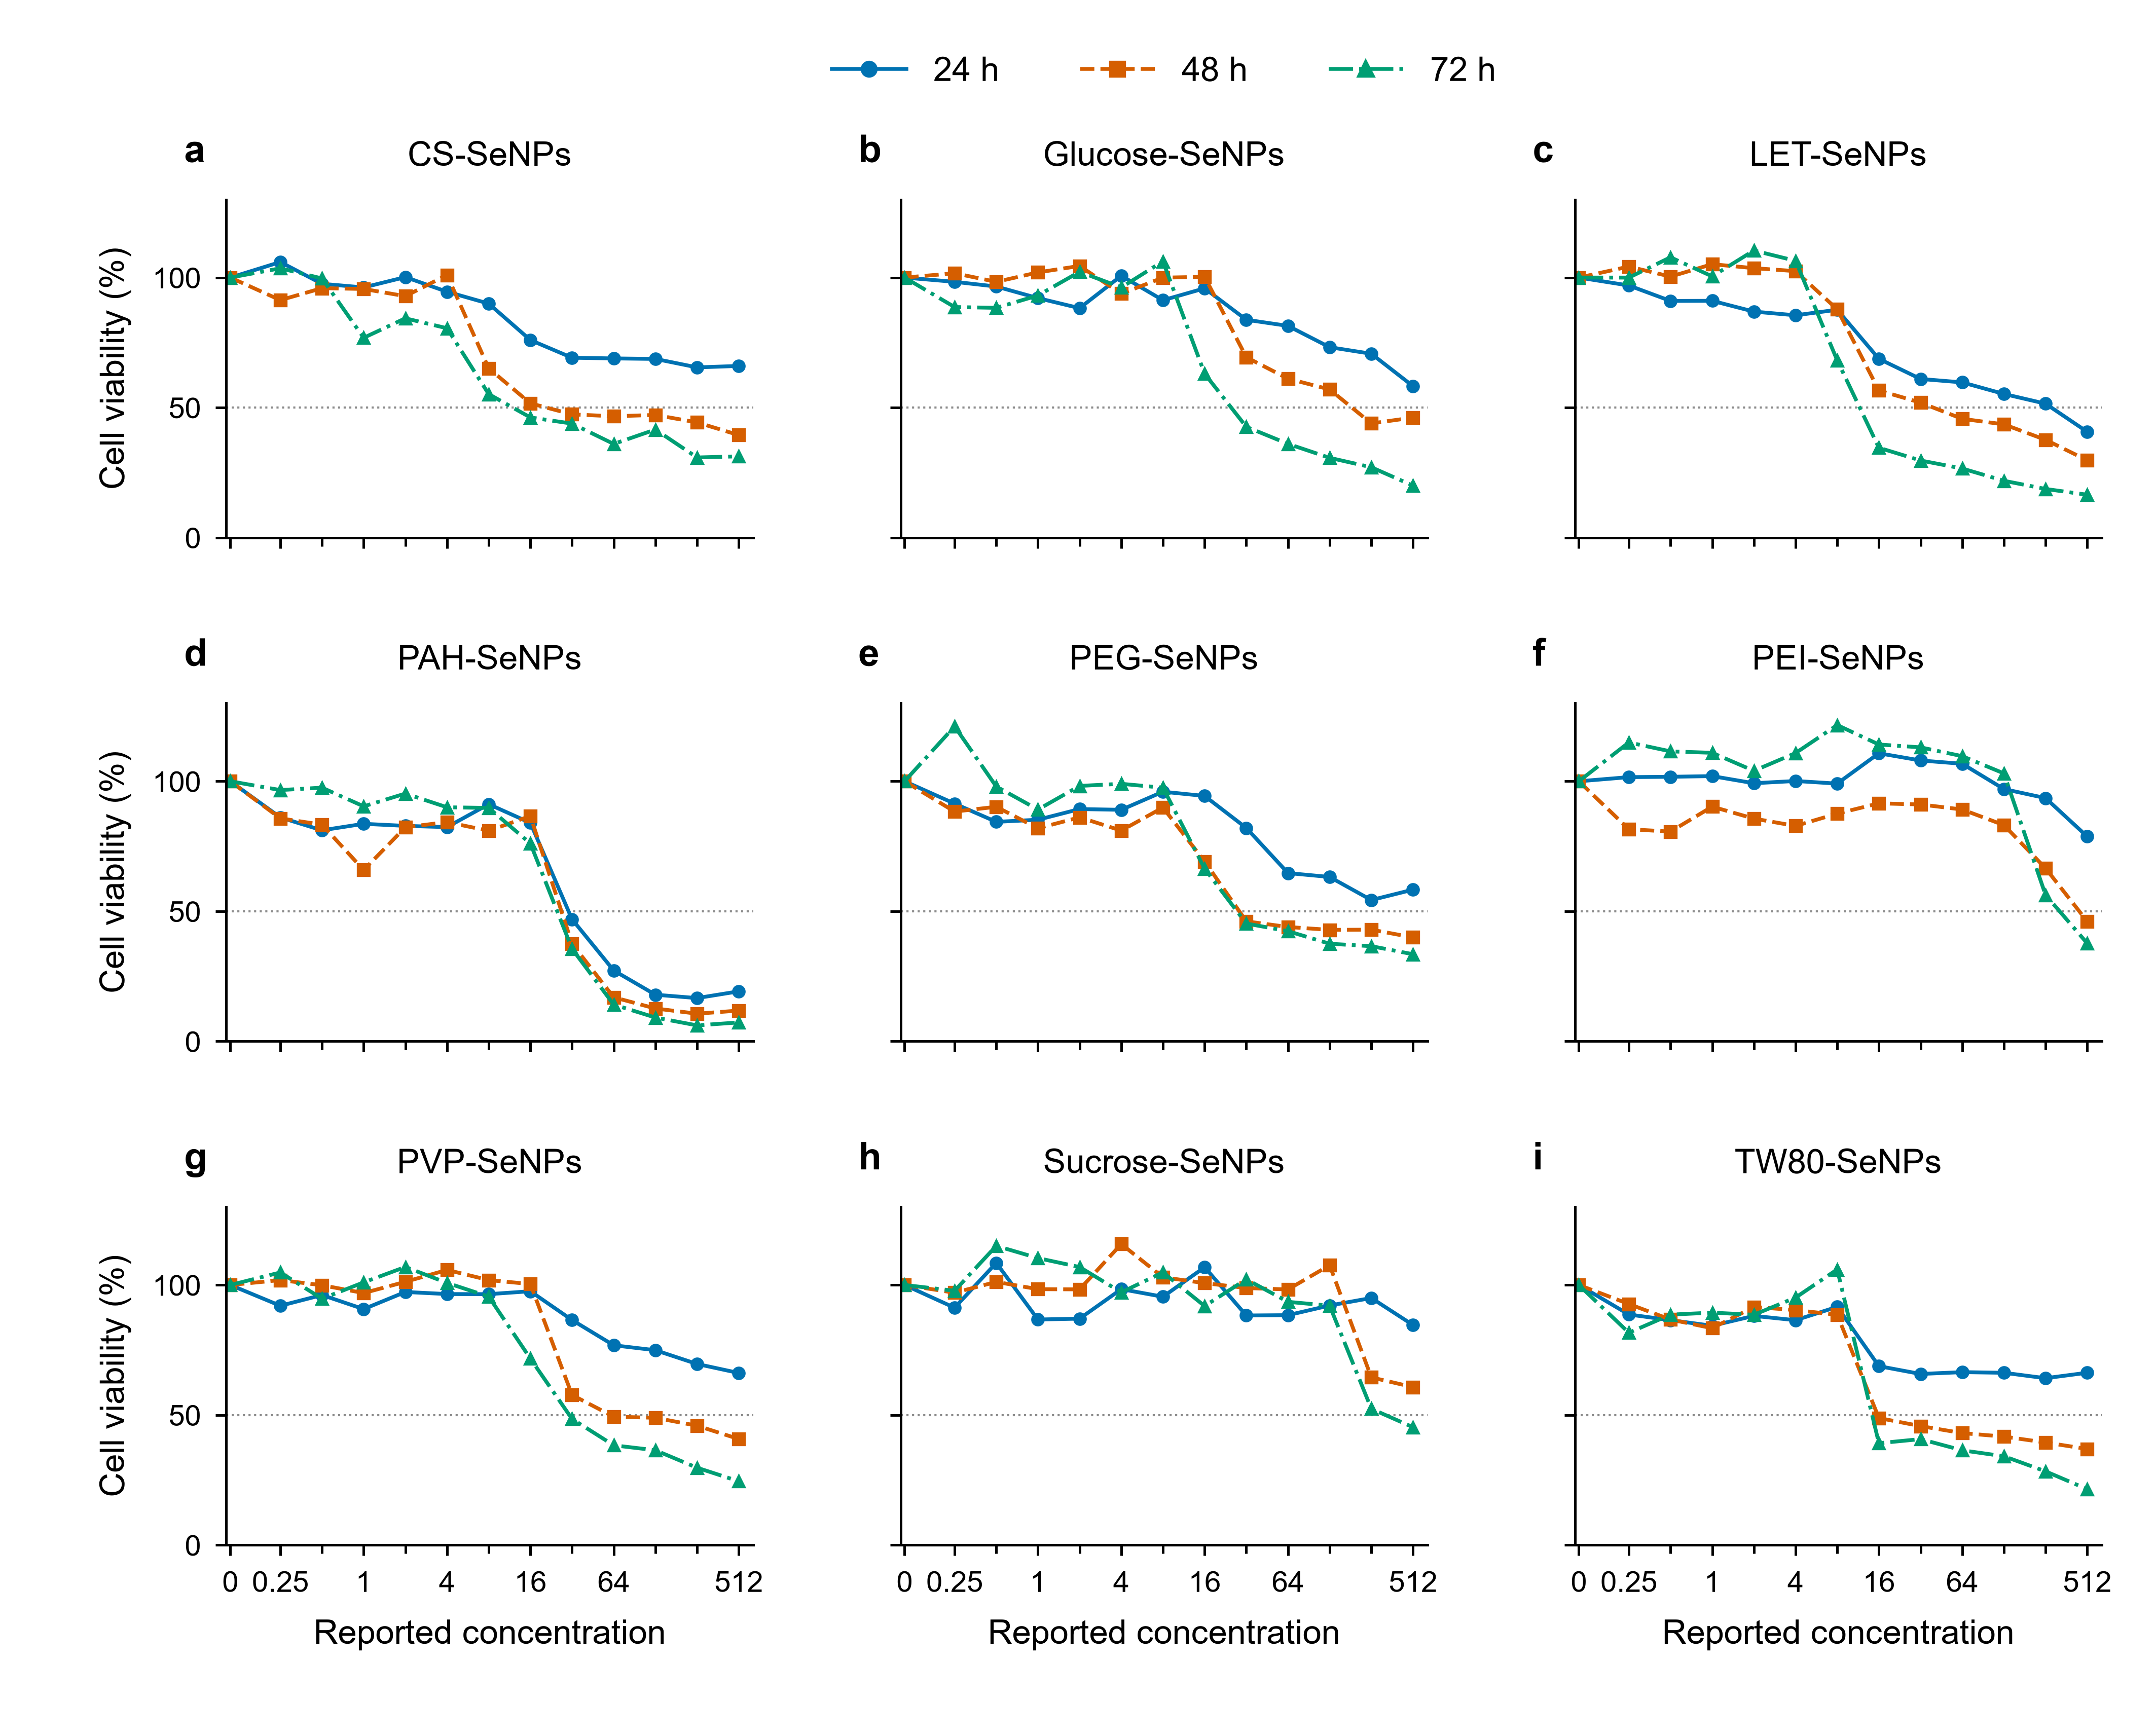
\includegraphics[width=\linewidth]{figures/huvec-dose-time.png}
\caption{9 种 SeNPs 在 HUVEC 中的剂量—时间报告曲线。a—i 依次为 CS、Glucose、LET、PAH、PEG、PEI、PVP、Sucrose 与 TW80，颜色、点形和线型区分 24、48、72 h。每条曲线包含 13 个报告点，横轴正浓度区采用以 2 为底的对数尺度，零点附近采用线性段以保留对照，浓度单位的含义与计量基准待核实。连线只连接报告点，灰色虚线表示 50\% 存活率；每个条件的重复次数与汇总方法未提供，图中不绘制误差条。}
\label{fig:huvec_dose_time}
\end{figure}

最高报告浓度 512 下，9 种材料的平均存活率在 24、48、72 h 分别为 59.81\%、39.07\% 和 26.38\%，24 h 至 72 h 下降 33.42 个百分点，九种材料在该浓度下均随时间延长而降低。该结果表明当前 HUVEC 观测具有高浓度下的时间依赖性，平均值描述的是不同材料的等权汇总，不是重复孔均值或实验误差估计。

在 HUVEC、72 h、报告浓度 512 下，PAH-SeNPs 的存活率最低，为 7.26\%，Sucrose-SeNPs 最高，为 45.30\%（表~\ref{tab:huvec_materials}）。其余材料按存活率递增依次为 LET、Glucose、TW80、PVP、CS、PEG 和 PEI，这一排序只描述指定条件下的观测差异，不代表所有剂量与时间下的统一安全性排序。

\begin{table}[htbp]
\centering
\caption{报告浓度 512 下的材料描述符与 HUVEC 存活率。按 72 h 存活率递增排列，每种材料的粒径和 Zeta 电位均为工作簿提供的固定报告值。}
\label{tab:huvec_materials}
\small
\begin{tabular}{lrrrrr}
\toprule
材料 & 粒径（nm） & Zeta（mV） & 24 h（\%） & 48 h（\%） & 72 h（\%） \\
\midrule
PAH-SeNPs & 190.72 & 51.70 & 19.21 & 11.82 & 7.26 \\
LET-SeNPs & 107.56 & \ensuremath{\mathord{-}}27.52 & 40.67 & 29.73 & 16.49 \\
Glucose-SeNPs & 115.82 & \ensuremath{\mathord{-}}23.83 & 58.25 & 46.16 & 19.98 \\
TW80-SeNPs & 78.03 & \ensuremath{\mathord{-}}21.90 & 66.26 & 36.93 & 21.48 \\
PVP-SeNPs & 143.76 & \ensuremath{\mathord{-}}31.79 & 66.16 & 40.78 & 24.52 \\
CS-SeNPs & 114.72 & 33.36 & 66.02 & 39.44 & 31.25 \\
PEG-SeNPs & 111.96 & \ensuremath{\mathord{-}}37.07 & 58.32 & 39.96 & 33.49 \\
PEI-SeNPs & 214.58 & 24.77 & 78.74 & 46.10 & 37.67 \\
Sucrose-SeNPs & 184.60 & 12.97 & 84.61 & 60.72 & 45.30 \\
\bottomrule
\end{tabular}

\end{table}

\subsection{表观 IC50 与描述符的探索性关联}

27 条曲线中，19 条存在唯一的相邻正浓度 50\% 括区，可得到表观 \IC，另外 8 条在测试范围内始终高于 50\%，记为 $>512$。可插值曲线在 24、48、72 h 分别为 2、8、9 条，有限估计在原始浓度尺度上为 11.63—448.56；完整结果见补充表~\ref{tab:huvec_ic50}，相邻点和状态保留在源数据表中。

表观 \IC 与最高浓度下的存活率描述不同的曲线特征，两者的材料排序并不完全一致。72 h 时，LET-SeNPs 的表观 \IC 最低，为 11.63，PAH-SeNPs 为 25.00，但 PAH-SeNPs 在报告浓度 512 下的存活率更低。对材料进行比较需要先明确评价时间、浓度范围和采用的曲线指标，不能将一个高浓度点的排序直接推广为全部剂量区间的排序。

在报告浓度 512 下，以 9 种材料为分析单位，粒径与 24、48、72 h 存活率的 Spearman 系数分别为 0.200、0.383 和 0.267，Zeta 电位对应值为 0.050、$-0.183$ 和 $-0.050$。这些描述性系数没有形成稳定的单变量关联证据，当前记录也不能区分粒径、电位、修饰化学及其他未测量因素的独立作用。新增实验尚未与事先封存的模型预测配对，因此这里不报告新材料预测的 MAE、RMSE、$R^2$、预测—实测排序相关或预测 \IC 误差。
\FloatBarrier

\section{讨论}

\subsection{预测问题的界定与材料信息的实际增量}

% Word body block 99
本研究把历史模型评价和新增实验观测置于同一研究问题下，同时保留两者不同的证据任务。历史分组结果显示，当前基础输入对跨文献存活率的预测仍有较大误差，更多化学字段、显式剂量—时间交互与固定预算迁移没有稳定降低误差；新增实验则提供了真实材料在 HUVEC 中的响应曲线，展示了时间变化与条件相关的材料差异。两部分共同说明，预测性能和实验响应结构需要各自获得直接证据，方向一致的实验趋势不足以替代逐样本预测评价。

% Word body block 100
化学增强的阴性结果限定于当前字段质量、样本组成与模型配置，并不说明材料化学性质在毒性形成中没有作用。历史数据的 Zeta 电位缺失率为 42.40\%，修饰物类别和分子量没有完整字段，晶体信息编码又只反映是否报告晶体学信息，这些条件限制了模型对材料差异的识别。表征方法、报告习惯和研究环境还可能共同影响输入值，新增字段是否具有生物学意义，与其能否在当前归档数据中提供稳定预测增量，属于需要分开讨论的问题。

% Word body block 101
同样，迁移对照尚未建立稳定收益，可能与不同材料体系的响应分布、共同特征的覆盖以及当前树模型迁移接口有关。RF 的新增树训练保留原有通用树，XGBoost 的续训依赖已学习的通用结构，本研究没有检验其他迁移方法，不能将结果推广为迁移学习对 SeNPs 普遍无效。对于现阶段的材料筛选，更合适的工作是明确模型可接受的输入、记录外部测试条件，并检验预测误差，而不是根据通用基准指标直接判断新材料预测精度。

\subsection{与既有计算研究的关系}

% Word body block 103
Gul 等的跨材料属性分析与 Masarkar 等的预测研究，为组织纳米材料理化性质、细胞背景和暴露条件提供了基础 [3, 4]。本研究进一步关注这些信息在 SeNPs 文献分组评价下的增量，以及新增实验如何与历史建模衔接。由于数据纳入、特征定义、模型选择与验证划分均不同，本研究不以跨论文的单个 R2 或 MAE 数值宣称性能优于既有工作，也不将归档中缺少完整训练证据的深度模型指标纳入当前主比较。

% Word body block 104
嵌套评价使内层选择与外层报告分离，对有限样本下模型选择偏差的控制与已有方法学研究一致 [5]。不过，文献分组验证只检验对未参与训练的文献组的表现，不能自动代表对未知配方、未知修饰物或不同实验室的泛化。旧历史复现还混合了随机交叉验证误差、全量拟合 R2 和不同预处理设置，当前结果不构成只改变划分方式的受控对照，因此性能差异不能全部归因于随机划分造成的泄漏，方法与数据口径的变化也需要保留在解释中。

\subsection{实验观测的意义与机制解释范围}

% Word body block 106
HUVEC 数据把研究从历史文献预测扩展到真实材料的剂量—时间观测，最高测试浓度下的时间变化与有限 IC50 估计数量的增加共同表明，评价时间会影响材料差异的呈现方式。对照已有SeNPs 细胞研究，这些结果支持将材料修饰和暴露条件一起纳入实验比较 [1, 2]，但当前单一细胞模型不能提供正常与肿瘤细胞选择性、跨细胞普适性或体内安全性的证据。

% Word body block 107
材料的高浓度排序与表观 IC50 排序并不一致，反映了固定浓度残余存活率与跨越 50\% 阈值所处位置的不同。表观 IC50 仅由两个相邻报告点插值，浓度间距、局部波动和检测读数都可能影响估计，尚不能用于给出精细的材料优劣判断。对没有跨越阈值的曲线保留 > 512 状态，也避免了在测试范围外强行拟合一个看似完整的数值。

% Word body block 108
粒径、电位和修饰信息在不同材料之间同时变化，每种材料又仅有一组描述符报告值，因此弱秩相关既不能证明这些性质无作用，也不能将某种材料的低存活率归因于单个描述符。大于 100\%的报告值同样需要谨慎解释，当前缺少原始孔读数、空白扣除及检测干扰信息，不能据此判定真实增殖促进或特定毒性机制。核对这些实验信息后，才能进一步评估剂量曲线的波动与材料相关的检测影响。

\subsection{外部预测评价仍需完成的环节}

% Word body block 110
冻结模型的逐条件预测文件具有解盲前封存记录，封存时间为 2026 年 10 月 13 日 16:23:13，记录的 SHA-256 与当前 model\_predictions.csv 一致。按材料、报告浓度、时间及浓度单位匹配后获得 351 对预测—实测值，因而本研究可以报告当前条件表上的 MAE、RMSE、平均偏差及预测—实测排序一致性。该评价仍受浓度单位及换算基准是否正确的影响，且每个条件只有一个归档报告值，不能据此估计独立实验重复间的变异。实测 IC50 不能作为新材料初筛模型的输入。

\section{结论}

本研究以文献分组嵌套评价重新界定历史 SeNPs 毒性预测的支持范围，并纳入 9 种材料在 HUVEC 中的完整剂量—时间报告数据。当前基础模型能够提供可复查的跨文献预测基准，化学增强、显式交互与固定预算迁移未显示稳定误差降低，含实测 \IC 的较低误差也不能替代新材料初筛的独立评价。

新增实验呈现了最高测试浓度下的时间依赖性和条件相关的材料差异，27 条曲线中 19 条可以估计表观 \IC，8 条在测试范围内没有达到 50\% 存活率。实验观测提高了研究的材料实证基础，但浓度单位、重复数据与操作记录仍需核实，当前尚未建立前瞻预测的配对误差或单一材料性质的因果解释。后续应用应以明确的输入条件、独立测试和可追溯实验记录为基础，再判断模型能否支持材料筛选与剂量范围选择。

\FloatBarrier
\section*{参考文献}

% Word body block 114
(1) Wang, H.; He, Y.; Liu, L.; Tao, W.; Wang, G.; Sun, W.; Pei, X.; Xiao, Z.; Jin, Y.; Wang,

% Word body block 115
M. Prooxidation and Cytotoxicity of Selenium Nanoparticles at Nonlethal Level in Sprague-

% Word body block 116
Dawley Rats and Buffalo Rat Liver Cells. Oxidative Medicine and Cellular Longevity 2020,

% Word body block 117
2020, 7680276, DOI: 10.1155/2020/7680276.(2) Lunkov, A.; Konovalova, M.; Shagdarova, B.; Zhuikova, Y.; Il’ina, A.; Varlamov, V. Synthesis

% Word body block 118
of Selenium Nanoparticles Modified by Quaternary Chitosan Covalently Bonded with Gallic

% Word body block 119
Acid. Polymers 2023, 15, 2123, DOI: 10.3390/polym15092123.(3) Gul, G.; Yildirim, R.; Ileri-Ercan, N. Cytotoxicity analysis of nanoparticles by association

% Word body block 120
rule mining. Environmental Science: Nano 2021, 8, 937–949, DOI: 10.1039/D0EN01240H.(4) Masarkar, A.; Maparu, A. K.; Nukavarapu, Y. S.; Rai, B. Predicting Cytotoxicity of Nanopar-

% Word body block 121
ticles: A Meta-Analysis Using Machine Learning. ACS Applied Nano Materials 2024, 7 ,

% Word body block 122
19991–20002, DOI: 10.1021/acsanm.4c02269.(5) Cawley, G. C.; Talbot, N. L. C. On Over-fitting in Model Selection and Subsequent Selection

% Word body block 123
Bias in Performance Evaluation. Journal of Machine Learning Research 2010, 11, 2079–2107.(6) Breiman, L. Random forests. Machine Learning 2001, 45, 5–32.(7) Chen, T.; Guestrin, C. In Proceedings of the 22nd ACM SIGKDD International Conference

% Word body block 124
on Knowledge Discovery and Data Mining, 2016, pp 785–794.

\clearpage
\appendix
\renewcommand{\thetable}{S\arabic{table}}
\setcounter{table}{0}
\section{补充材料}

\subsection{输入特征与参数候选}

% Word body block 127
基础配置的 19 个字段依次为：修饰/官能团信息、合成方法、表面电荷、细胞类型、细胞组织、发表年份、最终粒径、最终 Zeta 电位、Zeta 绝对值、暴露时间、历史浓度、log(1 + 粒径)、log(1 + 时间)、log(1 + 浓度)、接种细胞数，以及 Zeta、细胞数、修饰信息和表面电荷的四个缺失标志。化学候选为 Se 含量、稳定性时间、Se 3d 结合能和晶体学报告状态，IC50 配置额外考虑历史实测 IC50 。晶体学报告状态使用原晶体学字段是否非空构造，不是测定晶相的替代值。

% Word body block 128
RF 候选（树数、最大深度、叶节点最小样本数）为（250、不限、2）、（250、10、2）和（250、不限、4）；XGBoost 候选（轮次、最大深度、学习率）为（150、2、0.05）、（250、2、0.05）和（250、3、0.05）。固定预算通用与迁移对照使用 500 树预算，RF 的最小叶节点样本数为 2，XGBoost 的最大深度为 3、学习率为 0.05，其余固定参数与方法部分一致。

\subsection{完整配对增量结果}

% Word body block 130
表 S1 同时列出样本等权差值与文献组等权差值，区间对应后者。基础嵌套分析中归档的逐样本 bootstrap 指标区间属于另一不确定性口径，本稿不将它们写成文献组区间，也不将通用基准中的组等权区间直接附到样本等权性能数值上。

% Word body block 132: 表格逐单元格转写。
\begin{table}[H]
\centering
\caption{各配置相对对应基线的配对 MAE 差值，单位为存活率百分点。负值表示误差下降，区间来自 24 个文献组等权差值的 5000 次 bootstrap。}
\label{tab:paired_comparisons}
\small
\begin{tabularx}{\linewidth}{lXrrr}
\toprule
模型 & 对照 & \ensuremath{\Delta}MAE 样本等权 & \ensuremath{\Delta}MAE 文献组等权 & 文献组等权 95\% 区间 \\
\midrule
RF & 化学增强 & +0.180 & +0.183 & [0.054, 0.333] \\
XGBoost & 化学增强 & +0.030 & \ensuremath{\mathord{-}}0.049 & [\ensuremath{\mathord{-}}0.822, 0.668] \\
RF & IC50 辅助 & \ensuremath{\mathord{-}}0.142 & \ensuremath{\mathord{-}}0.326 & [\ensuremath{\mathord{-}}3.285, 2.542] \\
XGBoost & IC50 辅助 & \ensuremath{\mathord{-}}1.145 & \ensuremath{\mathord{-}}0.835 & [\ensuremath{\mathord{-}}3.296, 1.531] \\
RF & 加入剂量—时间交互 & +0.392 & +0.415 & [\ensuremath{\mathord{-}}0.072, 1.102] \\
XGBoost & 加入剂量—时间交互 & +0.605 & +0.388 & [\ensuremath{\mathord{-}}0.199, 1.016] \\
RF & General\ensuremath{\rightarrow}SeNP 迁移 & +0.577 & \ensuremath{\mathord{-}}0.535 & [\ensuremath{\mathord{-}}2.763, 1.414] \\
XGBoost & General\ensuremath{\rightarrow}SeNP 迁移 & \ensuremath{\mathord{-}}0.669 & \ensuremath{\mathord{-}}0.054 & [\ensuremath{\mathord{-}}1.417, 1.317] \\
\bottomrule
\end{tabularx}

\end{table}

\subsection{27 条曲线的表观 IC50}

% Word body block 135
表 S2 覆盖全部九种材料与三个时间点，不删除测试范围内未达到阈值的曲线。所有有限值均为对数浓度相邻点插值，单位沿用待核实的原始浓度尺度，显示两位小数仅用于一致排版，不表示相应的测量精度；> 512 只记录阈值未检出。该表不包含模型预测 IC50 或预测—实测误差。

% Word body block 137: 表格逐单元格转写。
\begin{table}[H]
\centering
\caption{HUVEC 材料—时间曲线的表观 IC50，采用原始浓度尺度。重复次数与汇总方法待核实。}
\label{tab:huvec_ic50}
\small
\begin{tabular}{lrrr}
\toprule
材料 & 24 h & 48 h & 72 h \\
\midrule
CS-SeNPs & $>512$ & 20.90 & 11.94 \\
Glucose-SeNPs & $>512$ & 185.33 & 24.89 \\
LET-SeNPs & 281.86 & 39.55 & 11.63 \\
PAH-SeNPs & 30.22 & 26.84 & 25.00 \\
PEG-SeNPs & $>512$ & 28.48 & 27.41 \\
PEI-SeNPs & $>512$ & 448.56 & 323.37 \\
PVP-SeNPs & $>512$ & 60.65 & 30.59 \\
Sucrose-SeNPs & $>512$ & $>512$ & 323.74 \\
TW80-SeNPs & $>512$ & 15.68 & 14.30 \\
\bottomrule
\end{tabular}

\end{table}

\subsection{新增实验源数据的使用规则}

% Word body block 140
新增实验原始报告字段为材料名称、粒径（nm）、Zeta 电位（mV）、细胞类型、浓度报告值、时间（h）和存活率（\%）351 条记录完整覆盖所有材料—时间—浓度组合，保留零浓度对照、60个大于 100\% 的存活率报告值与局部非单调响应，不做删点、额外归一化或浓度换算。材料比较表、时间汇总表、表观 IC50 的相邻括区与描述符相关系数均由归档 CSV 重新生成，原始工作簿与 CSV 的一致性以归档哈希及逐值核验为依据。

% Word body block 141
既有随机划分复现用于追溯历史报告，包含不同预处理和全量拟合指标，不进入本稿的主模型排名。原计划的修饰类别—分子量信息层级、可靠配方分组、完整材料表征与模型前瞻盲测，按当前归档可支持的范围记录，不将未生成的指标或未提供的数据补写为已完成结果。

\FloatBarrier
\section*{内部核验附录：暂不纳入正式正文的图件}

% Word body block 143
以下两张图随本轮材料一并保存，供作者核查，不应作为已验证的正式论文结果图直接投稿。IAE 热图的积分定义和完整计算脚本尚未核实。IC50 配对散点图中的预测 IC50 数值与逐条件预测曲线不一致：27 条预测曲线的最低预测存活率均高于 50\%，因此不能从当前预测曲线直接插值得到图中所示的有限模型 IC50。

% Word body blocks 144–145: 嵌入图保持原始字节。
\begin{figure}[H]
\centering
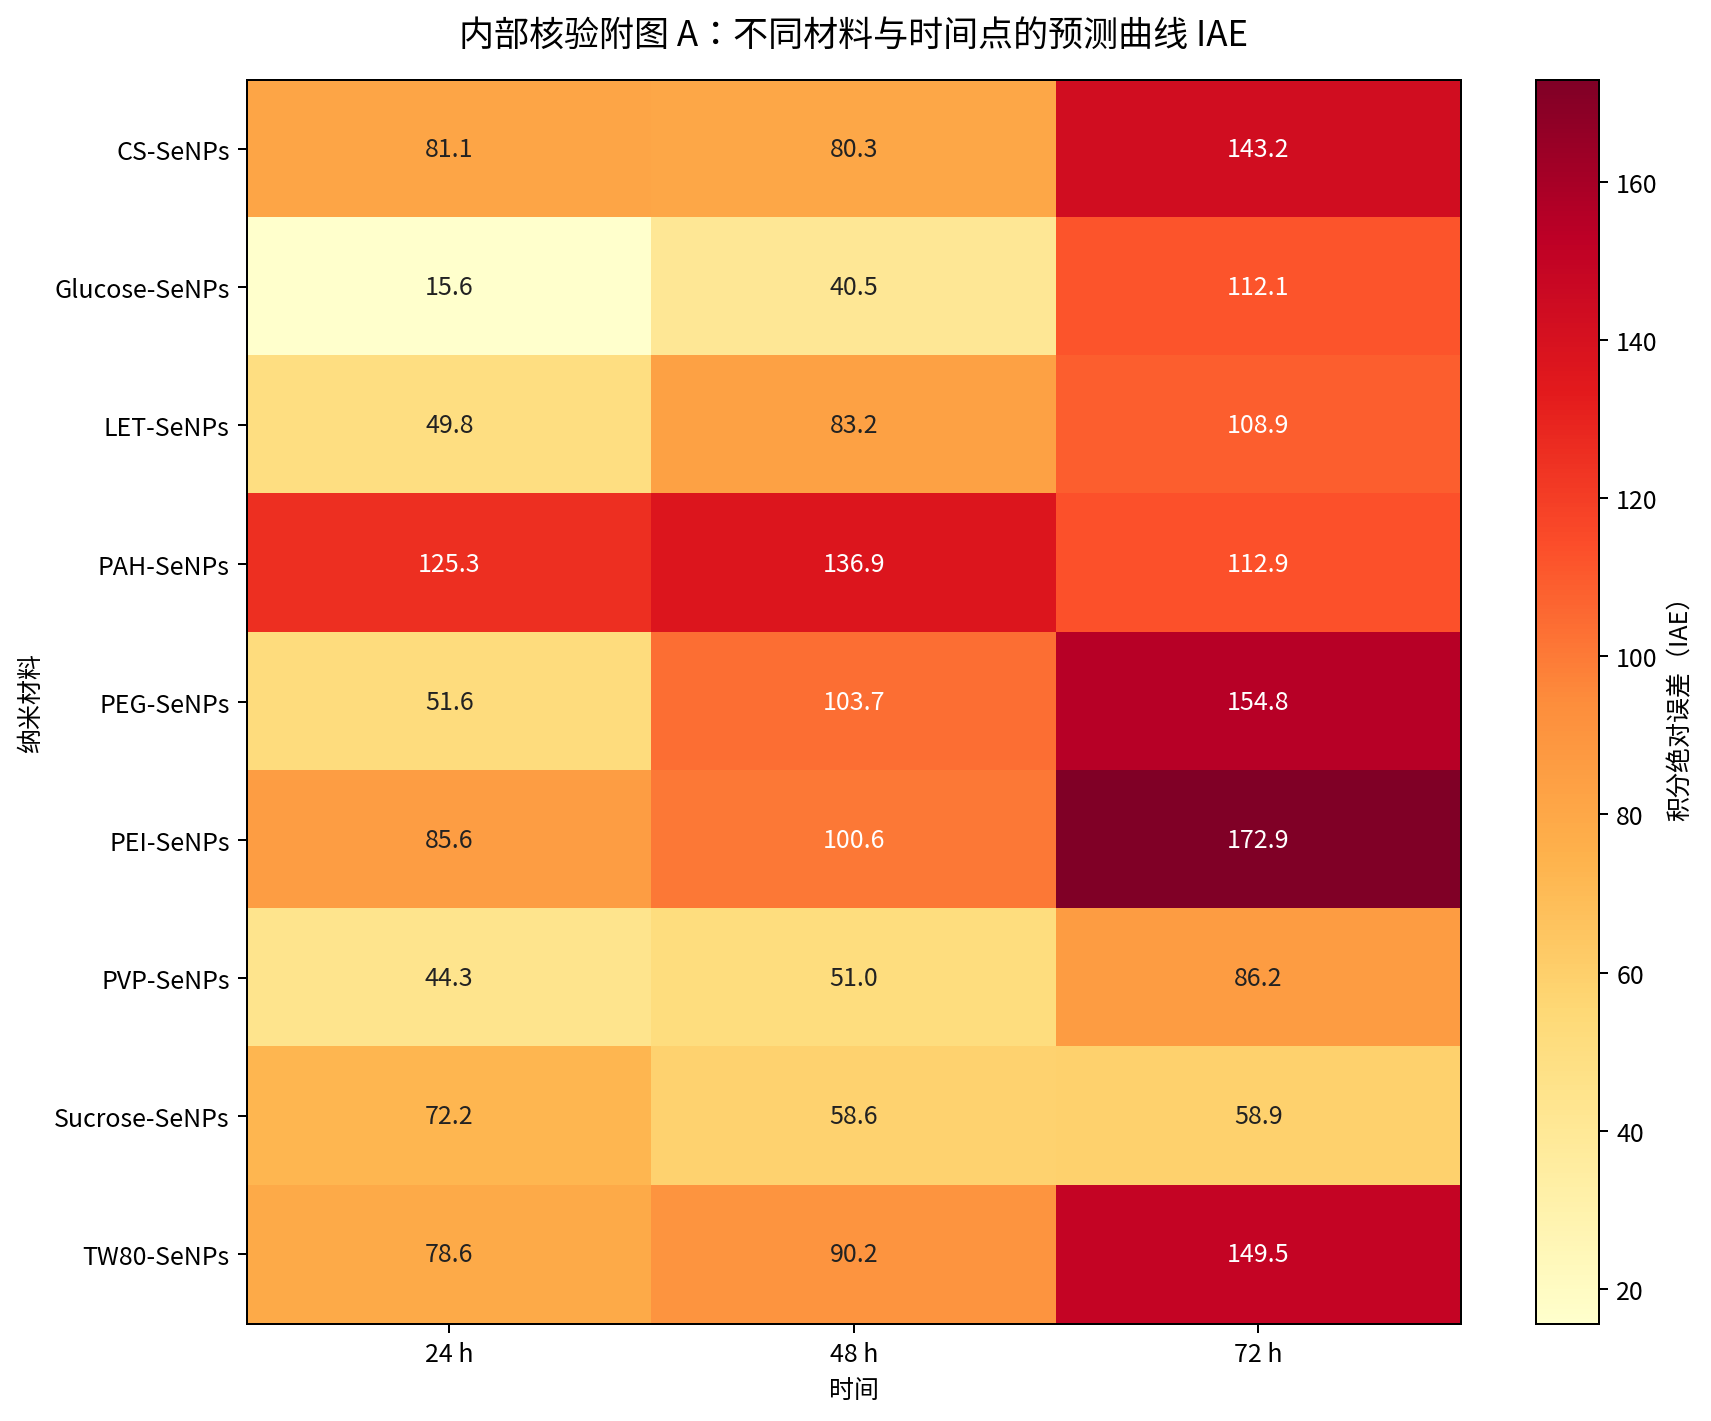
\includegraphics[width=\linewidth,height=0.70\textheight,keepaspectratio]{figures/word-20261021/iae-heatmap.png}
\caption*{内部核验附图 A. 任务 24 的 IAE 热图。暂不纳入正式正文，待核对积分横轴、零浓度处理、积分区间和数值积分方法后再决定。}
\label{fig:huvec_internal_iae}
\end{figure}

% Word body blocks 146–147: 嵌入图保持原始字节。
\begin{figure}[H]
\centering
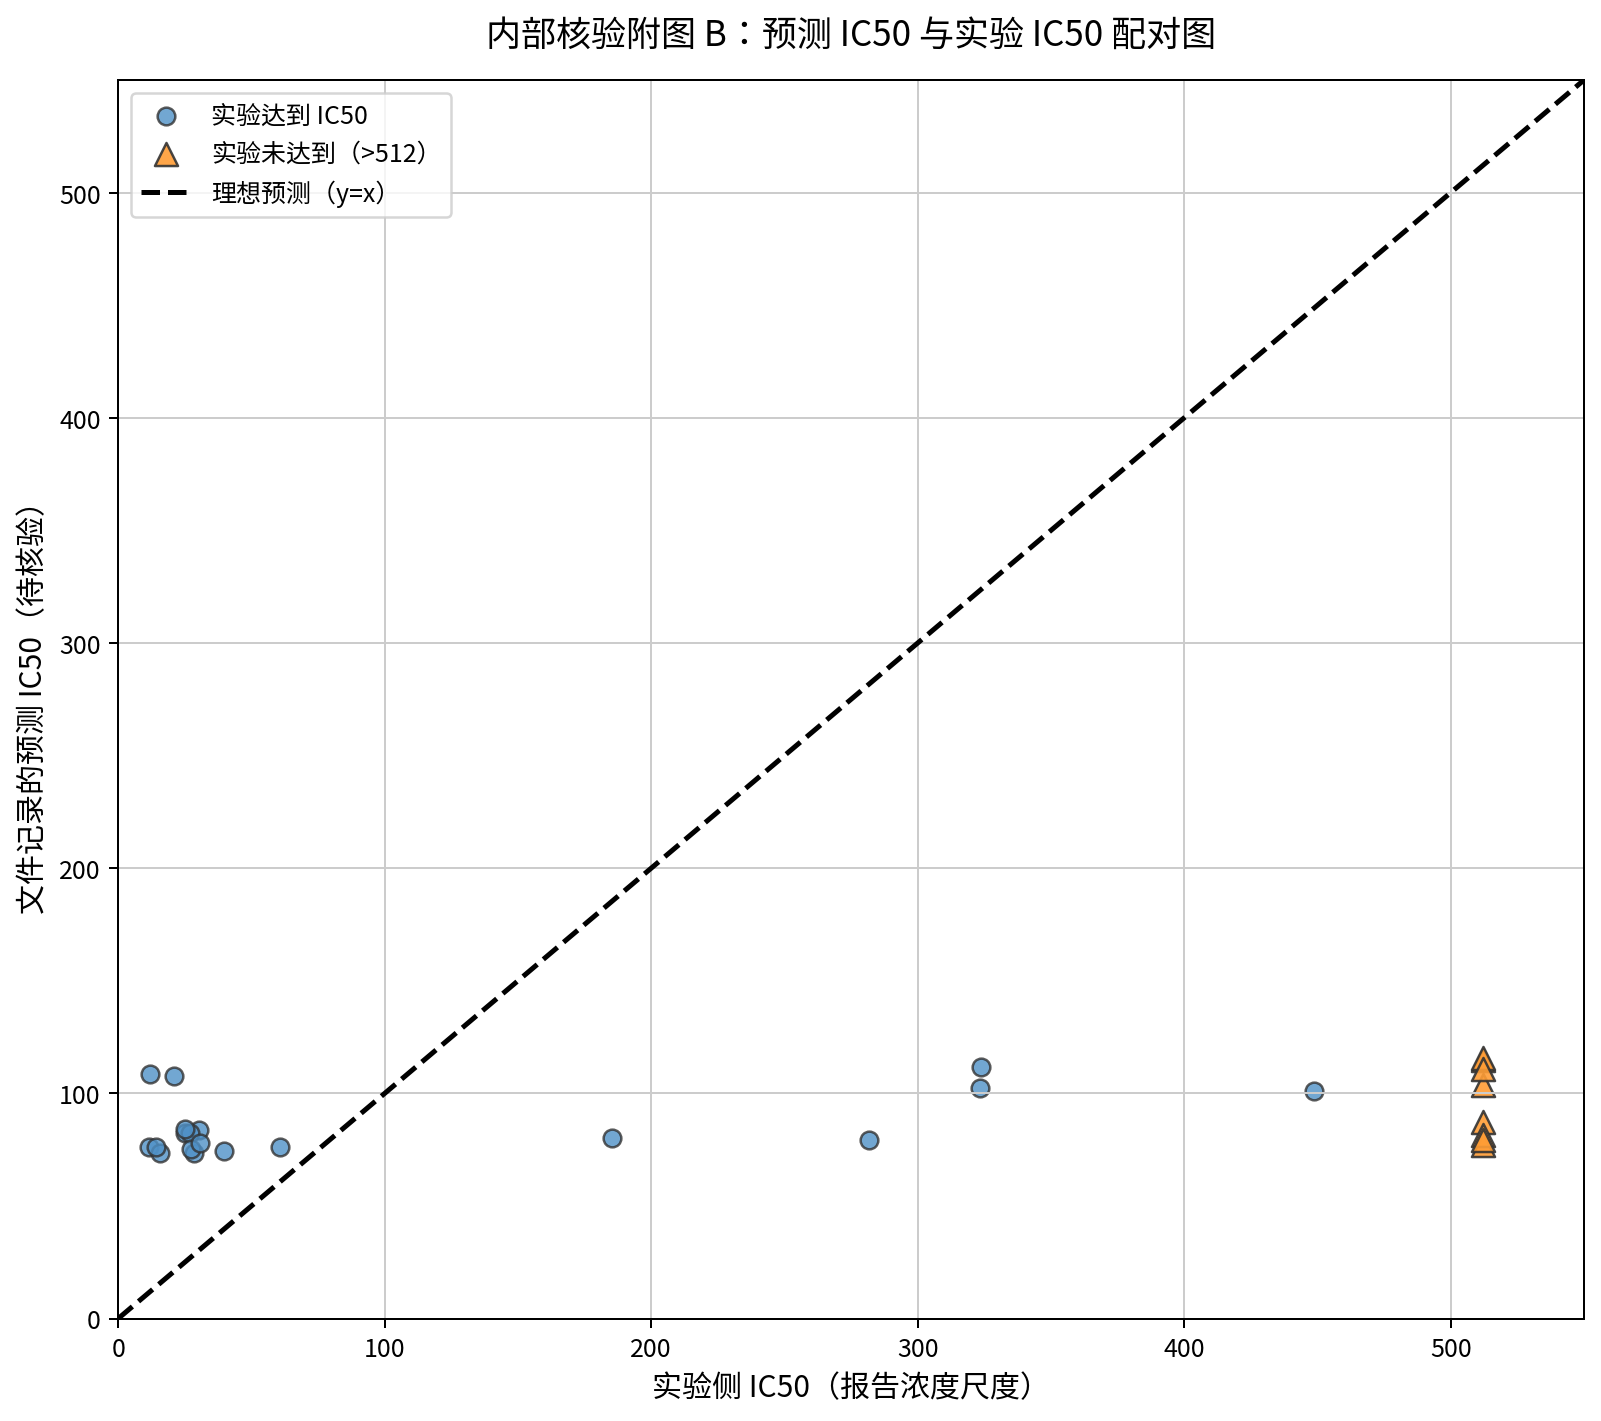
\includegraphics[width=\linewidth,height=0.70\textheight,keepaspectratio]{figures/word-20261021/ic50-pairing.png}
\caption*{内部核验附图 B. 预测 IC50 与实验 IC50 配对散点图。暂不纳入正式正文。预测曲线未跨越 50\% 存活率阈值，图中有限预测 IC50 及其配对误差目前缺少与曲线一致的可复现依据。}
\label{fig:huvec_internal_ic50}
\end{figure}

\subsection*{提交前仍需核验的事项}

% Word body block 149
核对实验浓度单位、元素硒计量基准及从报告浓度到模型输入浓度的换算方法。

% Word body block 150
补齐细胞来源、培养条件、检测方法、对照设置、归一化公式、技术重复和独立实验次数。

% Word body block 151
为 IAE 热图提供可复现的公式和计算脚本，并从预测—实测曲线重新计算。

% Word body block 152
移除或重新计算任务 26 中无法由预测曲线识别的 pred\_ic50、log\_error 及任何相关 R\textsuperscript{2}。

% Word body block 153
任务 30 的 SHAP 说明提到 shap\_code\_snippet.py，但当前附件中未提供该脚本正文。正式投稿前应随补充材料提供代码或稳定的代码存档入口。

\end{document}
